\chapter{Core Implementation}

%-------------------------------------------------------------------------------------------------------

\section{Building the Project}

\subsection{Obtaining the Source}
\noindent 
The latest version of the project's source code can be checked out via \textit{git} using: \\

\indent \textit{git clone https://github.com/swordmaster2k/botnav.git} \\

\noindent
Or downloaded as a ZIP file from \url{https://github.com/swordmaster2k/botnav}. \\ 

\noindent
Alternatively the most up to date version at the time of printing is available on the CD at the front of this thesis.

\subsection{Compiling the D* Lite Cython Module}
\noindent
The planning algorithm D* Lite must be compiled as a Cython module, the original source code was provided by Maxim Likhachev of CMU and Sven Koenig of USC in C. It has been modified to make it compatible with the core Python system using Cython, as Python is implemented in C \cite{•} it is inherently compatible with the sample of D* Lite that is provided by its authors.

\noindent
To build D* Lite you will need Python3.4, the Python3.4 headers, gcc, and make. It \textbf{must} be built for each platform on which it will execute as C compiles to machine code making it \textit{target dependent}. From a terminal navigate to the source code directory \textit{BotNav/algorithm/dstarlite\_build/}. \\

\noindent
The make file contains two build rules:
\begin{enumerate}
\item \textit{make} - \indent which builds the module \textit{dstarlite\_c.so} 
\item \textit{make clean} - \indent cleans all previous output files from the build process \\
\end{enumerate}

\noindent
Once the module file \textit{dstarlite\_c.so} has been successfully built for the target platform it can simply be dropped into the parent directory \textit{BotNav/algorithm/}. The Python source code contains a reference to the module and will automatically link it in at execution time. 

\subsection{Running it in Python3}
\noindent
By default the project is set-up to run a sample simulation with \textit{sample.map} using the GridNav path planning algorithm. It will output the results of its run to the \textit{BotNav/maps/output/} directory and is configured to compute a path from every traversable cell to the goal. To run it simply navigate to the path containing \textit{tester.py} and type: \\

\indent \textit{python3 tester.py config.botnav} \\

\noindent
The argument passed to \textit{tester.py} is the path to the default configuration file, the contents of which will be discussed later in this chapter. After running the above command in a terminal the result shall look similar to Figure \ref{sample_output}.

\begin{figure}[htbp]

\center 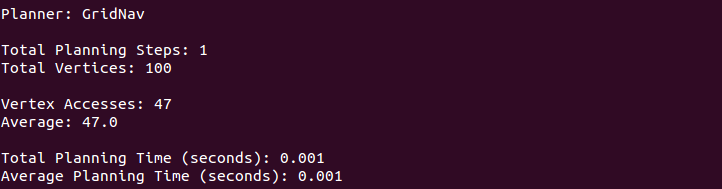
\includegraphics[width=435pt]{illustrations/sample_output}\\
\caption{An example of the type of output generated after running GridNav over \textit{sample.map} in simulation mode.} 
\label{sample_output}

\end{figure}

%-------------------------------------------------------------------------------------------------------

\section{Running Simulations}
\noindent
Simulations provide an easy means of testing each planning algorithm in controllable environments, it speeds up the testing process immeasurably, and provides reproduce-able results. The most powerful feature of simulations is the ability to plan a path from every free cell in the environment, the result of each traversal is placed into a separate timestamped folder. This data can then be easily mined and analysed in order to gauge how each algorithm performed for a particular scenario.

\subsection{Configuration}
\noindent 
When carrying out simulated runs three parameters must be set in the corresponding configuration file they are \textit{map}, \textit{mode}, and \textit{planner}. Below is an example of the configuration required to run a simulated trial using D* Lite: \\

	\indent \textit{map=maps/simple.map \\}
	\indent \textit{planner=d\_star\_lite \\}
	\indent \textit{mode=simulated \\}

\noindent
The most important parameter setting here is \textit{mode} which is set to simulated. At run time this informs the \textit{Tester} class that we want to run an experimental simulation across all traversable cells and that we do not need a communications channel via \textit{Proxy}. In simulation mode all of the instructions are invoked on the ``dummy'' robot class \textit{SimulatedRobot}, the method \textit{go\_to(self, x, y)} simply takes the $x$ and $y$ coordinates, introduces some random drift, and assigns them: \\

\begin{lstlisting}
def go_to(self, x, y):
	# Introduce a little uncertainty.
    self.x = (x + random.uniform(-0.2, 0.2)) * self.cell_size  
    self.y = (y + random.uniform(-0.2, 0.2)) * self.cell_size
    
    self.trail.append([self.get_cell_x(), self.get_cell_y()])
    
    self.state = "Travelled"
\end{lstlisting}

\subsection{Sample Output}

\begin{figure}[htbp]

\center 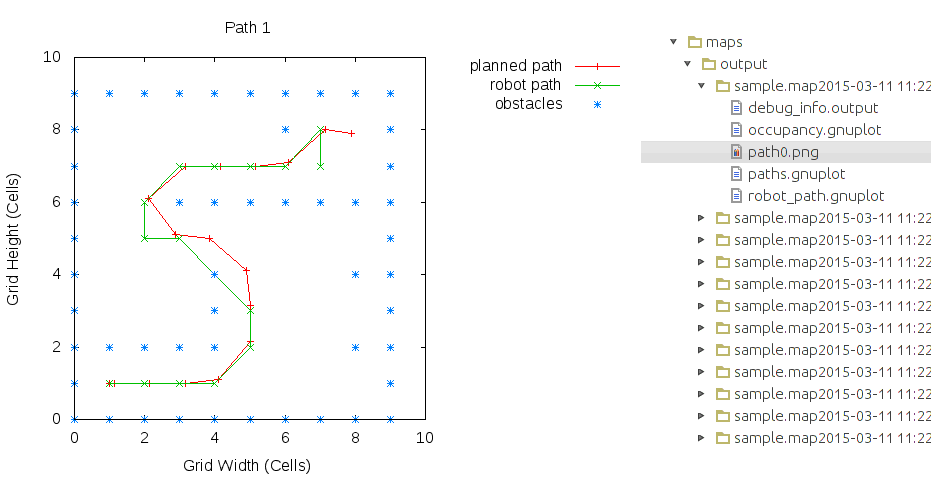
\includegraphics[width=435pt]{illustrations/sample_output_2}\\
\caption{A plot file for the first path from the sample map generated by \textit{gnuplot} (left), and the contents of the output folder after the run. Note that each folder is timestamped (right).} 
\label{sample_output}

\end{figure}

\newpage

%-------------------------------------------------------------------------------------------------------

\section{Using a Real Bot}
\noindent
The real test for any path planning algorithm is its practical effectiveness \cite{FIELD} and the only way to gauge this is using a physical robotic platform i.e.``a Real Bot''. The simulations that we have performed here are very limited in nature as they do not take into account any variability in the mechanics of the robot. While it is perfectly possible to model variations such as drift, odometry error, friction, and battery drain in a simulation it is far more practical to simply use a physical platform.  \\
  
\noindent
There are a number of factors that we must consider when using a physical robot, to begin with we will need some form of communications mechanism be it wired (USB, Ethernet, Serial) or wireless (ZigBee, WiFi, Bluetooth). It is through this medium that the \textit{Proxy} class will process the data to and from the robot. Then there is drift, occurrences such as wheel slippage can lead to the robot veering off course, we will assume that this issue is dealt with at a lower level than the path planning system.

\subsection{Configuration}
\noindent
The contents of the configuration file for a hardware robot depends on the communications medium being employed. At present the system supports three forms of communication Bluetooth, IP, and Serial. Before any of these can be used the run mode must set to \textit{physical}. Below is an example configuration using Bluetooth which requires the MAC address of the device and a port number: \\

	\indent \textit{map=maps/sample.map\\}
	\indent \textit{planner=grid\_nav\\}
	\indent \textit{mode=physical\\}
	\indent \textit{connection=bluetooth\\}
	\indent \textit{mac=00:00:12:06:56:83\\}
	\indent \textit{port=0x1001}
	
\noindent 
For IP based configurations an \textit{ip}, \textit{mac}, and \textit{port} setting will be required. Serial based connections need only a \textit{baud}, and \textit{port}, examples of both are available in the comments of the default configuration file: \\

	\indent \#   	\textit{if connection == bluetooth\\}
	\indent \#		\indent \textit{mac=\\}
	\indent \#      \indent \textit{port=\\}
	\indent \#   	\textit{elif connection == ip\\}
	\indent \#      \indent \textit{ip=\\}
	\indent \#      \indent \textit{mac=\\}
	\indent \#      \indent \textit{port=\\}
	\indent \#   	\textit{elif connection == serial\\}
	\indent \#      \indent \textit{baud=\\}
	\indent \#      \indent \textit{port=}

%-------------------------------------------------------------------------------------------------------

\section{How the Planner Works}
\noindent
As we have already seen our \textit{Planner} is implemented on its own separate thread which is designed to handle the bulk of the processing required to get our mobile robot from point a to b. All of this work is carried out within the \textit{run} method which is invoked when the thread is started. Below is a snippet of the code from the start of this method: \\

\begin{lstlisting}
'''
Step 1: Plan.
'''
self.algorithm.plan()

# Write the state after first planning step.
self.write_state()

# Append a copy of the path to our paths record.
paths.append(self.algorithm.path[:])

# Stick the starting position of the robot into
# the first path.
paths[0].insert(0, [self.robot.get_cell_x(), self.robot.get_cell_y()])

# Calculate our initial distance from the goal.
[output omitted]

# Write some debugging info.
self.write_debug_info()
\end{lstlisting}

\noindent
During the planning process the \textit{Planner} goes through a number of steps, part of the first step is outlined in the above code snippet. After the initial planning step that is used to evaluate if a path to the goal exists the planner immediately writes the state to our output files. Then some additions to the path collection are made including the robot's start position, the goal distance is calculated and checked, and lastly debugging information is recorded. This is just the first of five steps involved during the planning process this particular step only runs once per test. In the next section we will discuss all five steps together in \ref{steps}.

\subsection{Five Simple Steps}\label{steps}
\noindent
The planning process presented in this work was inspired by \cite{GRIDNAV95}. In \cite{GRIDNAV95} T. Balch established a simple methodology that enabled a mobile robot equipped with grid based planner to successfully navigate towards its goal in an iterative manner using seven steps. Those steps can be seen on page 7 of his paper. Our planning process was originally derived from these steps and later simplified by reducing it from seven steps to five:

\newpage

\begin{enumerate}
\item Plan.
\item Scan the immediate area for obstacles and free space.
\item Update the map if necessary.
\begin{enumerate}
\item Recompute the plan if necessary.
\end{enumerate}
\item Pop the next point from the current path and travel.
\item Go to 2.
\end{enumerate}

\noindent
In the original version the initialisation of variables and the reading of the map file were included as a step, this is not included in the \textit{Planner} directly so it was removed. Also step 5 from \cite{GRIDNAV95} became the optional step 3(a) as this step will only ever be taken if the condition for step 3 becomes \textit{true}. This process will iteratively execute from step 2 through 5 until either the goal is reached \textit{or} when no path can be found. Essentially all of the work in this entire project evolved from this methodology. By reading over \cite{GRIDNAV95} we can gain a fundamental understanding of everything that grid based path planning involves from start to finish. 

\subsection{Abstracting Away from the Algorithm}
\noindent
Art the heart of the object oriented patterns used in this project is \textit{abstraction}, a technique that enables a developer to generalise the functionality of a class through abstract inheritance. Through this process the complexity of an object can be reduced and its efficiency greatly increased \cite{http://whatis.techtarget.com/definition/abstraction}. It has been used extensively in the implementation of the path planning algorithms which all inherit from the base class \textit{AbstractAlgorithm}. From this class each algorithm inherits a series of default behaviours some of which are listed here:

\newpage

\begin{itemize}
\item plan(self) -
\item pop\_next\_point(self) -
\item update\_occupancy\_grid(self, cells) - 
\item print\_debug(self, stream) - 
\end{itemize}

\noindent
The real advantage to using abstraction here is the \textit{pluggable} nature it provides. Every algorithm that inherits from the \textit{AbstractAlgorithm} base class implements a common set of behaviours and properties. Regardless of which algorithm is currently being used for planning we simply access the same behaviour or property (see Figure \ref{abstraction_method}). The implementation details of each algorithm is hidden from the \textit{Planner} whom only cares about the results.

\begin{figure}[htbp]

\center 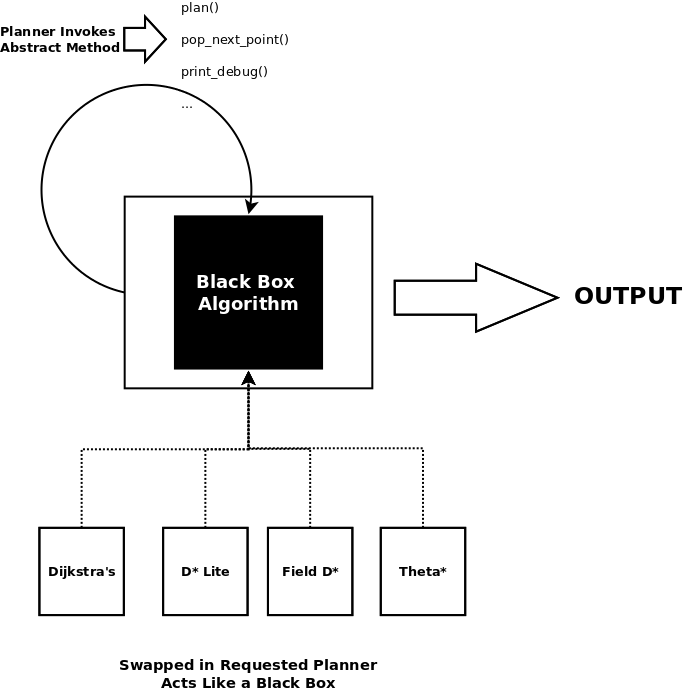
\includegraphics[width=290pt]{illustrations/abstraction}\\
\caption{The current algorithm acts as a black box to the \textit{Planner} whom calls a set of public abstract methods. Any planning algorithm can be swapped in for testing without having to account for any implementation specifics.} 
\label{abstraction_method}

\end{figure}

%-------------------------------------------------------------------------------------------------------

\newpage

%\section{Open Field D*}
%Core of the project very important, state that every implementation of Field D* to date is closed source NASA's code is %not available, nor is Carnegie Mellon's. Open Field D* is significant because it bucks this trend making it open to ITB %students and others.

%\subsection{Modifying D* Lite}
%Point out the key differences between D* Lite and Field D* from a coding perspective, nodes to cell corners how this is %represented, linear interpolation. Using Georgia Institute of Technologies D* Lite code state the modifications %required to get Field D*.

%\subsection{Basic Implementation}
%Cover basic implementation of Field D*, most importantly state any problems encountered, or variations/optimisations %made during the coding stage.

%-------------------------------------------------------------------------------------------------------